\documentclass[12pt,letterpaper]{article}
\usepackage{geometry}
\geometry{
    top=35mm, bottom=30mm, left=25mm, right=25mm, headheight=35mm
}
\usepackage{graphicx}
\usepackage{titling}
\usepackage{enumerate}
\usepackage{float}
\usepackage{fancyhdr}
\usepackage{blindtext}
\usepackage{lipsum}
\usepackage[spanish]{babel}
\pagestyle{fancy}
\usepackage{array}
\usepackage{tabularx}
\usepackage{colortbl}
\usepackage{bigstrut}
\usepackage{lmodern}
\usepackage{setspace}
\usepackage{wrapfig}
\usepackage{tikz}
\usepackage{imakeidx}
\usepackage{times}
\definecolor{rosa}{RGB}{255, 146, 214}
\definecolor{jaja}{RGB}{30, 41, 250}
\definecolor{green}{RGB}{166,212,162}

\lhead{
    
\includegraphics[width=0.35\linewidth]{logo_largo.png}
}
\rhead{
    \textcolor{jaja}{\textbf{Agile Programming Innovators S.R.L.}}\\
    No.1785, C/ J.C. Canedo, Cercado,\\
    Cochabamba, Bolivia, 0000\\
    E-mail: api.programming.company@gmail.com
}
\author{Agile Programming Innovators S.R.L.}
\title{\textbf{Entregable de QA \\ API}}

\include{format}
\makeindex

\begin{document}

\begin{titlepage}
    \begin{center}
        \vspace*{1cm}

        
\includegraphics[width=0.4\textwidth]{logo.png}
        
        \vspace{1cm}
        \Huge
        \textbf{Informe de QA de Software}
        
        \small
        Versión 4
            
            
        \vspace{0.5cm}
        \Large
        \textbf{Agile Programming Innovators}        
            
        \vspace{1cm}
               
        \Large
        Departamento de Informática y Sistemas\\
        Universidad Mayor de San Simón\\
        Cochabamba, Bolivia\\
        Octubre 2024

        \vfill

        \small
        © Copyright 2024 by\\
        \large
        \textbf{The Institute of Software Engineering Workshop, TIS}\\
       \textbf{ 354 Oquendo Street, Cochabamba, CB 0000, BO.}\\

        \vspace{1cm}
        
       \small
       \textit{Prohibida la reproducción total o parcial de esta publicación por cualquier medio,}\\
       \textit{en un sistema electrónico de recuperación o de otro modo,}\\
       \textit{sin autorización previa del editor.}\\
            
    \end{center}
\end{titlepage}
\newpage

\tableofcontents
\listoffigures
\listoftables
\newpage

%%%%%%%%%%%%%%%%%%%%%%%%%%%%%%%%%%%%%%%%%%%%%%%%%%%%%%%%%%%%%%

\section{Garantía}

Acorde al contrato se debe cumplir con los objetivos establecidos en la adenda \textit{AD - 01 - 2024} + los objetivos establecidos en el sprint 2, considerando la existencia de una boleta de garantía y todas las implicaciones que esta conlleva.

\section{Introducción}

    \subsection{Descripción de la audiencia}
    
    La audiencia prevista está compuesta por usuarios con experiencia previa en el desarrollo y uso de software. Se trata de un público más técnico, familiarizado con conceptos de programación, que busca información detallada sobre el funcionamiento interno del producto.

    \subsubsection{Nivel de experiencia esperado}
    \begin{itemize}
        \item Se espera que el usuario tenga conocimientos intermedios o avanzados en desarrollo de software, manejo de bases de datos, y sistemas de control de versiones.
        \item El usuario debería ser capaz de entender términos técnicos relacionados con flujo de trabajo en desarrollo ágil, además de poder interpretar código y documentación técnica.
    \end{itemize}
    
    \subsubsection{Formación previa}
    \begin{itemize}
        \item Se asume que el usuario tiene formación en ciencias de la computación, ingeniería de software, o una carrera afín.
        \item Experiencia en la implementación de sistemas similares y conocimiento de lenguajes de programación utilizados en el desarrollo del producto son recomendables. Usuarios con experiencia en frameworks o plataformas específicas también se beneficiarán de una mejor comprensión del producto.
    \end{itemize}
    
    \subsection{Declaración de aplicabilidad}
    
    Este documento contiene la primera versión del informe Quality Assurance (QA), el entorno de trabajo para esta versión es un servidor local con carácterísticas mínimas hardware de 2 GB de memoría RAM y 20 GB espacio en disco.
    
    \subsection{Declaración de propósito}

    \subsubsection{Verificar la Funcionalidad del Software:}
        Asegurar que todas las funcionalidades del software cumplen con los requisitos especificados y funcionan según lo esperado.
        
    \subsubsection{Evaluar la Estabilidad y Confiabilidad:}
    Identificar posibles defectos y problemas de estabilidad del software bajo diferentes condiciones de uso.
    
    \subsubsection{Evaluar el Rendimiento del Software:}
    Medir el rendimiento del software (tiempos de respuesta, uso de recursos, etc.) para asegurar que cumpla con los estándares y expectativas de los usuarios.
    
    \subsubsection{Identificar y Documentar Defectos:}
    Registrar todos los defectos y problemas encontrados durante las pruebas para su posterior corrección.
    
    \subsubsection{Asegurar la Conformidad con los Estándares:}
    Validar que el software cumple con las normativas y estándares de calidad aplicables al proyecto.
    
    \subsubsection{Proveer Recomendaciones para Mejoras:}
    Sugerir mejoras y optimizaciones basadas en los hallazgos durante el proceso de QA, contribuyendo a un software más robusto y eficiente.
    
    
    \subsection{Descripción del uso del documento}

    El documento contiene las siguientes secciones:
    \begin{itemize}
        \item Metodología de Pruebas, para determinar los tipos de pruebas, herramientas y las estrategias utilizadas. 
        \item Planificación de pruebas, para determinar el cronograma de etapa de pruebas, especificar los roles del equipo de testing.
        \item Ejecución de pruebas, en esta sección se encuentran las validaciones de los tests realizados.
    \end{itemize}
    
    \subsection{Lista o información de documentos relacionados}

    Este es el primero documento de una serie de documentos que sobre Quality Assurance para el desarrollo del proyecto TISTracker.
    
    \subsection{Instrucciones de reporte de problemas}

    Si se encuentra algún problema relacionado con el funcionamiento del software o la documentación, te agradecemos que lo informes para poder solucionarlo de manera oportuna. Sigue las siguientes instrucciones para reportar problemas o sugerir mejoras:

    \begin{itemize}
        \item  Asegúrate de proporcionar una descripción detallada del problema. Incluye información sobre las acciones que realizaste antes de que ocurriera el error, los mensajes de error (si los hay), y el entorno en el que sucedió (sistema operativo, navegador, versión del software).
        \item Si es posible, adjunta archivos de registro, capturas de pantalla o cualquier otra información relevante que nos ayude a reproducir y analizar el problema.
        \item Si puedes, incluye una lista de pasos que sigues para reproducir el error.
    \end{itemize}
    
    \subsection{Alcance de las Pruebas}
    Para esta primera entrega preveremos que las pruebas puedan ser suficientes para probar las funcionalidades de las historia de usuario comprometidas.

%%%%%%%%%%%%%%%%%%%%%%%%%%%%%%%%%%%%%%%%%%%%%%%%%%%%%%%%%%%%%%
%%%%%%%%%%%%%   DESDE AQUI ES EL CUERPO DEL DOCUMENTO %%%%%%%%
%%%%%%%%%%%%%%%%%%%%%%%%%%%%%%%%%%%%%%%%%%%%%%%%%%%%%%%%%%%%%%

\section{Metodología de Pruebas}

    \subsection{Tipos de Pruebas Realizadas}
    Pruebas de Características (Feature Tests):
    Estas pruebas verifican la funcionalidad completa de una característica del sistema, incluyendo la interacción con la base de datos, las rutas y los controladores.
    
    Pruebas Funcionales (Functional Testing): Se enfocan en comprobar que el software cumple con los requisitos funcionales especificados.

    Pruebas de Usabilidad (Usability Testing): Verifican la facilidad de uso del software para los usuarios finales.

    Pruebas de Usuario (User Acceptance Testing - UAT): Realizadas en colaboración con los usuarios finales para validar si el software cumple con sus expectativas y necesidades.

    Pruebas de Exploración (Exploratory Testing): Realizadas sin un guión de pruebas estricto, estas pruebas permiten al QA explorar el sistema en busca de comportamientos inesperados o errores.
    
    \subsection{ Herramientas y Técnicas Utilizadas}
    \subsubsection{Azure Devops}
    Se uso Devops para identificar los tets case en función a las criterios de aceptación de las historias de usuario.
    \subsubsection{Backend (Laravel)}
    PHPUnit es un framework de pruebas unitarias para PHP. Se utiliza para escribir y ejecutar pruebas unitarias y de características en el backend.

    \subsubsection{Laravel Sanctum:}
    Laravel Sanctum proporciona un sistema ligero de autenticación de tokens para SPAs (aplicaciones de una sola página), aplicaciones móviles y APIs simples.

\subsection{Estrategia de Pruebas (Manual vs. Automatizadas)}
\subsubsection{Backend}
    En el backend en se han implementado:
    Pruebas de Características (Feature Tests)
    Estas pruebas verifican la funcionalidad completa de una característica del sistema, incluyendo la interacción con la base de datos, las rutas y los controladores que se ejecutan de manera automática.

\subsubsection{FrontEnd}
    Para el frontend, se implementó una estrategia de pruebas manuales llevadas a cabo por un especialista en Quality Assurance (QA). Este enfoque incluye:
    Pruebas Exploratorias
    El QA realiza pruebas exhaustivas de la interfaz de usuario, explorando diferentes escenarios y flujos de usuario para identificar posibles errores o inconsistencias en la experiencia del usuario.
    Pruebas de Usabilidad
    Se evalúa la facilidad de uso, la intuitividad y la eficiencia de la interfaz, asegurando que cumpla con los estándares de diseño y las expectativas del usuario.
    Pruebas de Compatibilidad
    El QA verifica el funcionamiento correcto de la aplicación en diferentes navegadores y dispositivos, garantizando una experiencia consistente para todos los usuarios.
    Pruebas de Aceptación del Usuario (UAT)
    El QA simula escenarios de uso real para validar que la aplicación cumple con los requisitos del negocio y las expectativas del usuario final.
%%%%%%%%%%%%%%%%%%%%%%%%%%%%%%%%%%%%%%%%%%%%%%%%%%%%%%%%%%%%%%

\section{Planificación de Pruebas}


    
    \subsection{Roles y Responsabilidades}
    \subsubsection{QA Encargado:}
    Simón Eduardo Abasto Martinis\\
    \subsubsection{QA designado}\\
    
    \begin{enumerate}
        \item Ricardo Rojas carvajal
        \item Erwin Antonio Paredez Castro
    \end{enumerate}
    
    
 
\subsection{Criterios de Entrada y Salida}
\subsubsection{Criterios de Entrada}
    Para iniciar las pruebas de QA, se deben cumplir los siguientes criterios:
    \begin{itemize}
    \item El equipo de desarrollo ha completado la implementación de las funcionalidades por HU planificadas en el sprint.
    \item El entorno de pruebas está configurado y es accesible, con un servidor local que cumple los requisitos mínimos (2 GB de memoria RAM y 20 GB de espacio en disco).
    \item Los casos de prueba están definidos y documentados en Azure DevOps.
    \item Las herramientas necesarias para las pruebas (PHPUnit, Laravel Sanctum) están instaladas y configuradas.
    \end{itemize}


\subsubsection{Criterios de Salida}
    Para considerar completado el proceso de QA, se deben cumplir los siguientes criterios:
    \begin{itemize}
    \item Todos los casos de prueba definidos han sido ejecutados.
    \item Las pruebas de características (Feature Tests) en el backend han sido completadas y pasadas satisfactoriamente.
    \item Las pruebas manuales en el frontend, incluyendo pruebas exploratorias, de usabilidad, y de compatibilidad, han sido realizadas.
    \item Todos los defectos críticos y de alta prioridad han sido identificados y documentados.
    \item Se ha completado el análisis de los resultados de las pruebas.
    \item Se ha generado un informe detallado de QA que incluye métricas de calidad, resumen de defectos y recomendaciones.
    \item El equipo de QA ha validado que la aplicación cumple con los criterios de aceptación definidos en las historias de usuario.
    \end{itemize}
    
%%%%%%%%%%%%%%%%%%%%%%%%%%%%%%%%%%%%%%%%%%%%%%%%%%%%%%%%%%%%%%








\section{Ejecución de Pruebas}

    \subsection{Casos de Prueba y Resultados Cary Over}
    
    %4--
    \subsubsection{Registrarse a grupo TIS}
    \begin{figure}[H]
        \centering
        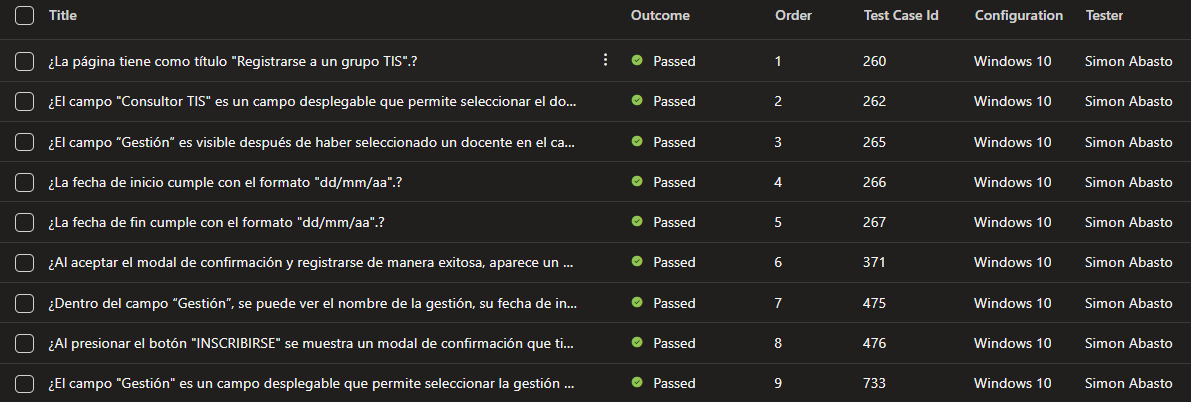
\includegraphics[width=1\linewidth]{case unirse a grupo de gestion proyectos tis.png}
        \caption{Test points Unirse a grupo de gestión de proyectos Tis}
    \end{figure}


\begin{table}[h] % Agrega un entorno de tabla
    \centering % Para centrar la tabla en la página
    \caption{Registrarse a grupo TIS} % Agrega la caption aquí
     \begin{tabular}{|c|c|c|c|c|c|}
       \rowcolor{green} % Color de la primera fila
    \hline
    Test plan name & Test points & Run \% & Passed \% & Failed \% & Not run count \\
    \hline
    Registrarse a grupo TIS    & 9   & 100   & 100     & 0    & 0    \\
    \hline
    \end{tabular}
    \end{table}



%5-
\subsubsection{Ver solicitud de creación de grupo empresa}
 \begin{figure}[H]
        \centering
        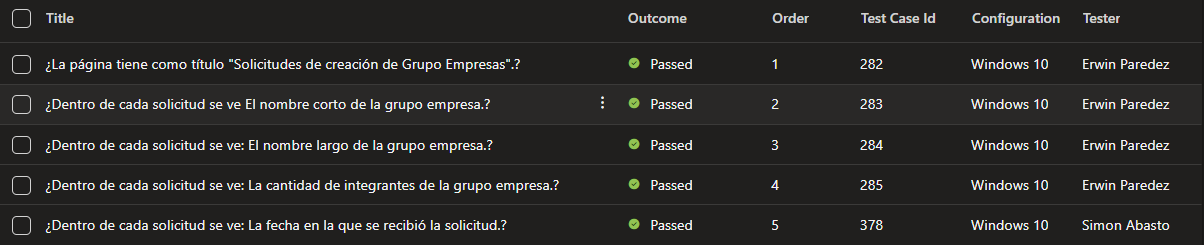
\includegraphics[width=1\linewidth]{cases ver solicitud de creacion de grupo empresa.png}
        \caption{Test points Ver solicitud de creación de grupo empres}
    \end{figure}


\begin{table}[h] % Agrega un entorno de tabla
    \centering % Para centrar la tabla en la página
    \caption{Ver solicitud de creación de grupo empresa} % Agrega la caption aquí
     \begin{tabular}{|c|c|c|c|c|c|}
       \rowcolor{green}% Color de la primera fila
    \hline
    Test plan name & Test points & Run \% & Passed \% & Failed \% & Not run count \\
    \hline
    Ver solicitud de creación de grupo empresa    & 5    & 100   & 100    & 0    & 0    \\
    \hline
    \end{tabular}
    \end{table}

%%%%%%%%%%%%%%%%%%%%%%%%%%%%%%%%%%%         %%%%%%%%%%%%%%%%%%%%%%%%%%%%%%%%%%%%%%%%%









%9-
\subsubsection{Confirmar integrantes grupo empresa}
\begin{figure}[H]
        \centering
        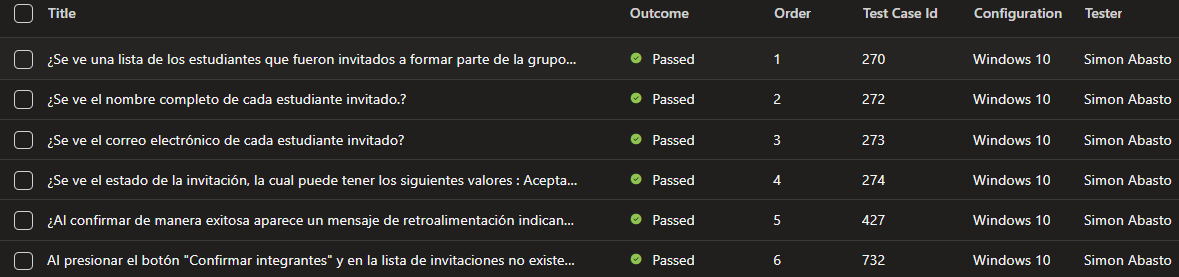
\includegraphics[width=1.1\linewidth]{cases confirmar integrantes de grupo empresa.png}
        \caption{Test points Confirmar integrantes grupo empresa}
    \end{figure}


 \begin{table}[h] % Agrega un entorno de tabla
    \centering % Para centrar la tabla en la página
    \caption{Confirmar integrantes grupo empresa} % Agrega la caption aquí
    \begin{tabular}{|c|c|c|c|c|c|}
        \rowcolor{green} % Color de la primera fila
        \hline
        Test plan name & Test points & Run \% & Passed \% & Failed \% & Not run count \\
        \hline
        Confirmar integrantes grupo empresa & 5 & 100 & 100 & 0 & 0 \\
        \hline
    \end{tabular}
\end{table}







%10-
\subsubsection{Ver invitaciones de grupo empresa}
\begin{figure}[H]
        \centering
        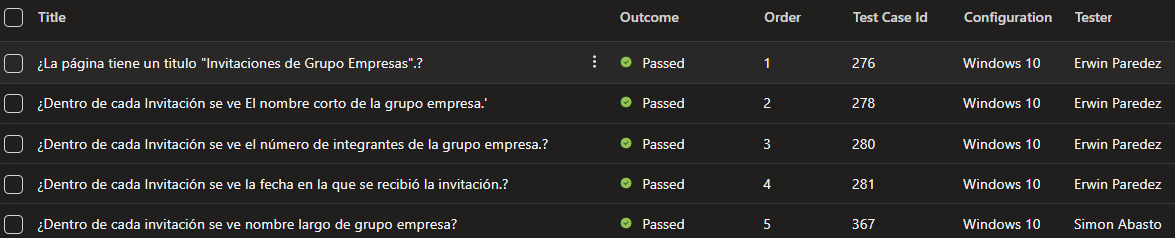
\includegraphics[width=1.1\linewidth]{cases ver invitaciones de grupo empresa.png}
        \caption{Test points Ver invitaciones de grupo empresa}
    \end{figure}


 \begin{table}[h] % Agrega un entorno de tabla
    \centering % Para centrar la tabla en la página
    \caption{Ver invitaciones de grupo empresa} % Agrega la caption aquí
    \begin{tabular}{|c|c|c|c|c|c|}
        \rowcolor{green} % Color de la primera fila
        \hline
        Test plan name & Test points & Run \% & Passed \% & Failed \% & Not run count \\
        \hline
        Ver invitaciones de grupo empresa & 7 & 100 & 100 & 0 & 0 \\
        \hline
    \end{tabular}
\end{table}


%11-
\subsubsection{Aceptar/rechazar conformación de grupo empresa}
\begin{figure}[H]
        \centering
        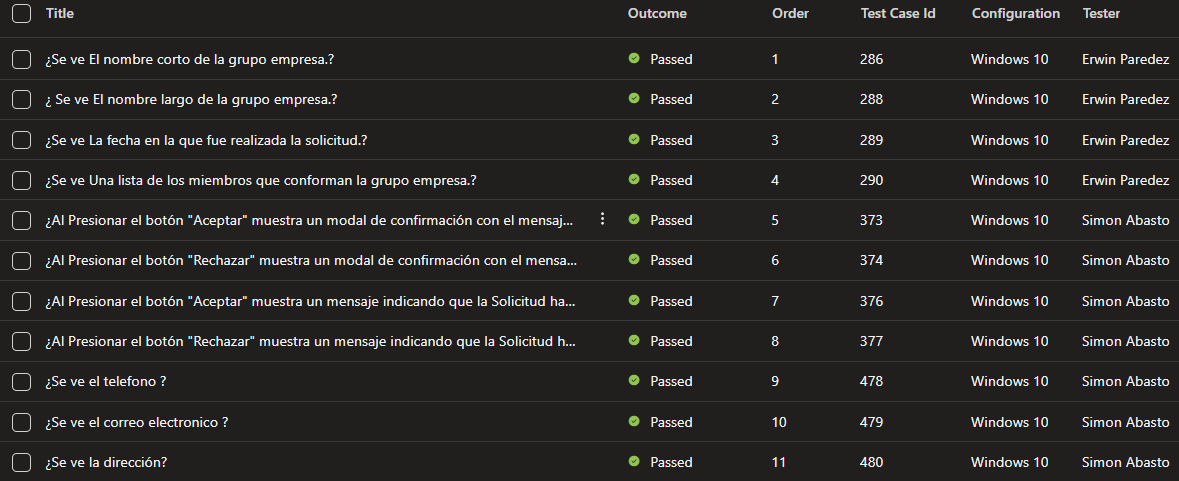
\includegraphics[width=1\linewidth]{cases aceptar conformacion de grupo empresa.png}
        \caption{Test points Aceptar conformación de grupo empresa}
    \end{figure}


 \begin{table}[h] % Agrega un entorno de tabla
    \centering % Para centrar la tabla en la página
    \caption{Aceptar conformación de grupo empresa} % Agrega la caption aquí
    \begin{tabular}{|c|c|c|c|c|c|}
        \rowcolor{green} % Color de la primera fila
        \hline
        Test plan name & Test points & Run \% & Passed \% & Failed \% & Not run count \\
        \hline
        Aceptar conformación de grupo empresa& 11 & 100 & 100 & 0 & 0 \\
        \hline
    \end{tabular}
\end{table}



%12-
\subsubsection{Aceptar/Rechazar invitación de una grupo empresa}

\begin{figure}[H]
        \centering
        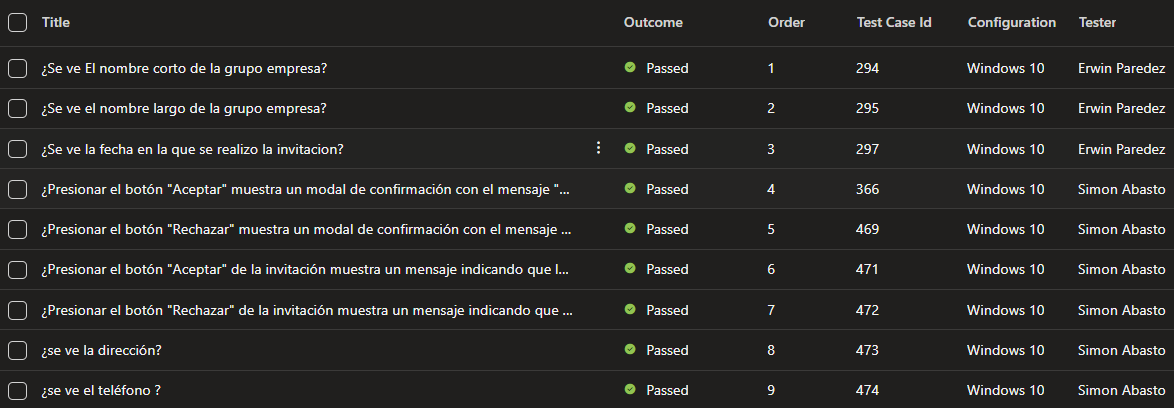
\includegraphics[width=1\linewidth]{cases aceptar inivtacion de un grupo empresa.png}
        \caption{Test points Aceptar invitación de una grupo empresa}
    \end{figure}


 \begin{table}[h] % Agrega un entorno de tabla
    \centering % Para centrar la tabla en la página
    \caption{Aceptar invitación de una grupo empresa} % Agrega la caption aquí
    \begin{tabular}{|c|c|c|c|c|c|}
        \rowcolor{green} % Color de la primera fila
        \hline
        Test plan name & Test points & Run \% & Passed \% & Failed \% & Not run count \\
        \hline
        Aceptar invitación de una grupo empresa& 9 & 100 & 100 & 0 & 0 \\
        \hline
    \end{tabular}
\end{table}



%13-
\subsubsection{Retirar invitación a grupo empresa}
\begin{figure}[H]
        \centering
        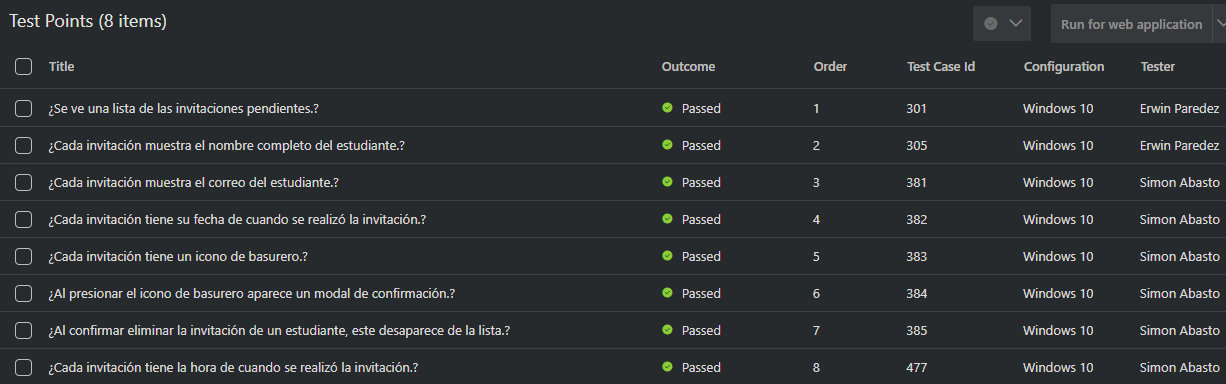
\includegraphics[width=1\linewidth]{cases retirar invitacion a grupos empresa.png}
        \caption{Test points Retirar invitación a grupo empresa}
    \end{figure}


 \begin{table}[h] % Agrega un entorno de tabla
    \centering % Para centrar la tabla en la página
    \caption{Retirar invitación a grupo empresa} % Agrega la caption aquí
    \begin{tabular}{|c|c|c|c|c|c|}
        \rowcolor{green} % Color de la primera fila
        \hline
        Test plan name & Test points & Run \% & Passed \% & Failed \% & Not run count \\
        \hline
        Retirar invitación a grupo empresa& 8 & 100 & 100 & 0 & 0 \\
        \hline
    \end{tabular}
\end{table}



%14-
\subsubsection{Enviar invitación a estudiante para unirse a la grupo empresa}
\begin{figure}[H]
        \centering
        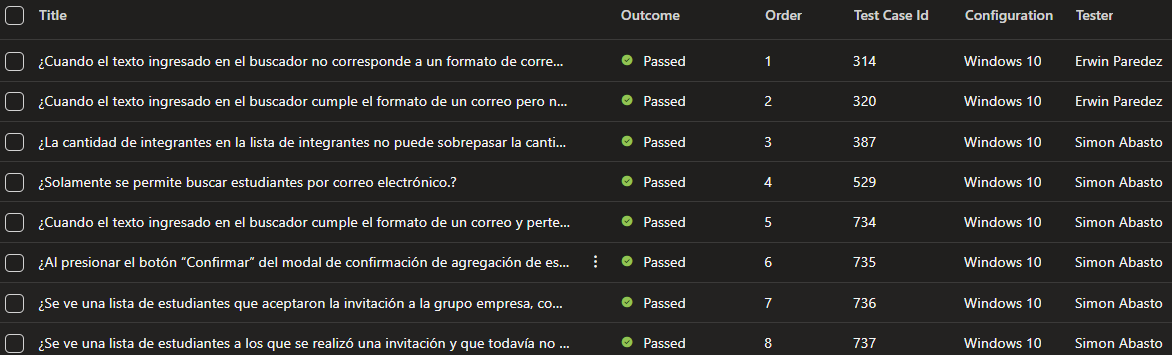
\includegraphics[width=1\linewidth]{cases enviar invi.png}
        \caption{Test points Enviar invitación a estudiante para unirse a la grupo empresa}
    \end{figure}

 \begin{table}[h] % Agrega un entorno de tabla
    \centering % Para centrar la tabla en la página
    \caption{Enviar invitación a estudiante para unirse a la grupo empresa} % Agrega la caption aquí
    \begin{tabular}{|c|c|c|c|c|c|}
        \rowcolor{green} % Color de la primera fila
        \hline
        Test plan name & Test points & Run \% & Passed \% & Failed \% & Not run count \\
        \hline
    invitación a estudiante para unirse a la GE& 8& 100 & 100 & 0 & 0 \\
        \hline
    \end{tabular}
\end{table}


%%Sprint 3 % ---------------------------------------------------------------------------------------------------------------------------------------------------------------------------------------------------



%-
\subsubsection{Ver grupo empresa para seguimiento semanal}
\begin{figure}[H]
        \centering
        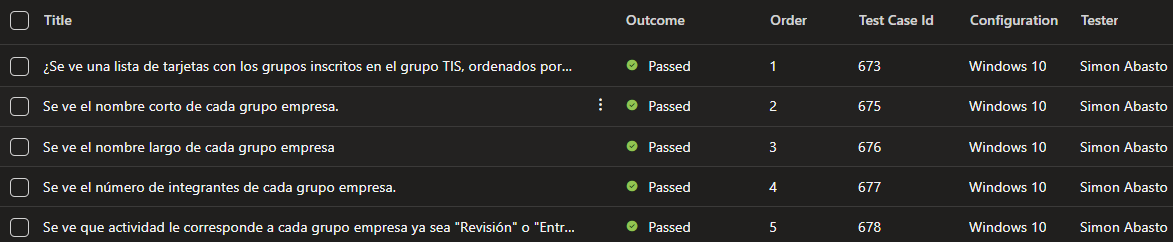
\includegraphics[width=1\linewidth]{Ver grupo empresa para seguimiento semanal.png}
        \caption{Test points Ver grupo empresa para seguimiento semanal}
    \end{figure}

 \begin{table}[h] % Agrega un entorno de tabla
    \centering % Para centrar la tabla en la página
    \caption{Ver grupo empresa para seguimiento semanal} % Agrega la caption aquí
    \begin{tabular}{|c|c|c|c|c|c|}
        \rowcolor{green} % Color de la primera fila
        \hline
        Test plan name & Test points & Run \% & Passed \% & Failed \% & Not run count \\
        \hline
   Ver grupo empresa para seguimiento semanal& 5 & 100 & 100 & 0 & 0 \\
        \hline
    \end{tabular}
\end{table}

%%Sprint 4 % ---------------------------------------------------------------------------------------------------------------------------------------------------------------------------------------------------



\subsubsection{Ver reportes de evaluaciones semanales}
\begin{figure}[H]
        \centering
        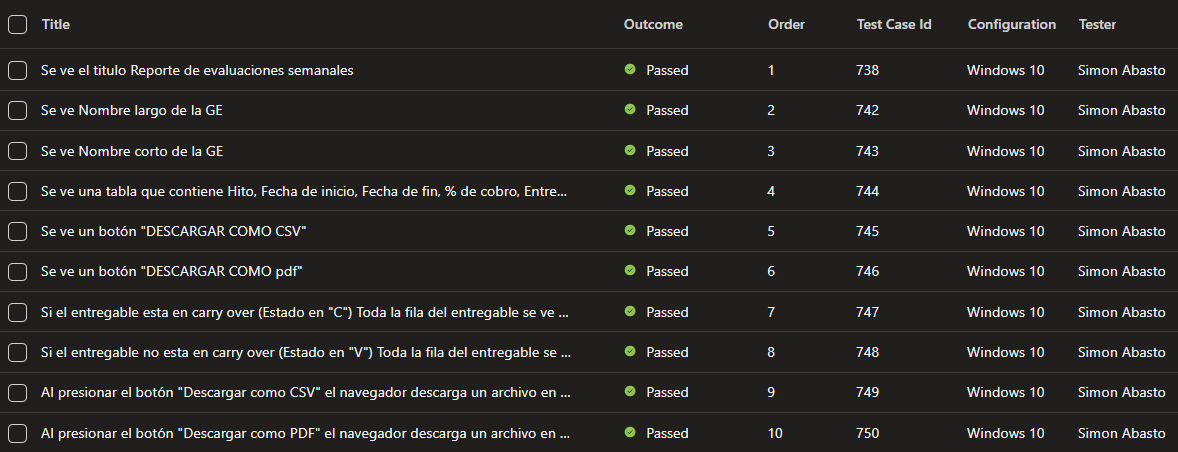
\includegraphics[width=1\linewidth]{Ver reportes de evaluaciones semanales.png}
        \caption{Test points Ver reportes de evaluaciones semanales}
    \end{figure}

 \begin{table}[h] % Agrega un entorno de tabla
    \centering % Para centrar la tabla en la página
    \caption{Ver reportes de evaluaciones semanales} % Agrega la caption aquí
    \begin{tabular}{|c|c|c|c|c|c|}
        \rowcolor{green} % Color de la primera fila
        \hline
        Test plan name & Test points & Run \% & Passed \% & Failed \% & Not run count \\
        \hline
  Ver reportes de evaluaciones semanales& 10 & 100 & 100 & 0 & 0 \\
        \hline
    \end{tabular}
\end{table}


\subsubsection{Ver reportes de calificaciones de estudiantes}
\begin{figure}[H]
        \centering
        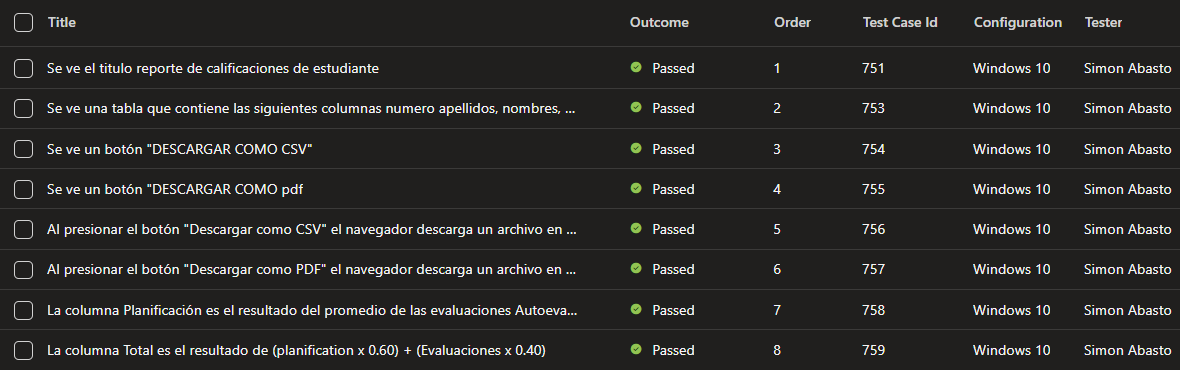
\includegraphics[width=1\linewidth]{Ver reportes de calificaciones de estudiantes.png}
        \caption{Test points Ver reportes de calificaciones de estudiantes}
    \end{figure}

 \begin{table}[h] % Agrega un entorno de tabla
    \centering % Para centrar la tabla en la página
    \caption{Ver reportes de calificaciones de estudiantes} % Agrega la caption aquí
    \begin{tabular}{|c|c|c|c|c|c|}
        \rowcolor{green} % Color de la primera fila
        \hline
        Test plan name & Test points & Run \% & Passed \% & Failed \% & Not run count \\
        \hline
   Ver reportes de calificaciones de estudiantes& 8 & 100 & 100 & 0 & 0 \\
        \hline
    \end{tabular}
\end{table}


\subsubsection{Ver reportes de calificaciones de GE}
\begin{figure}[H]
        \centering
        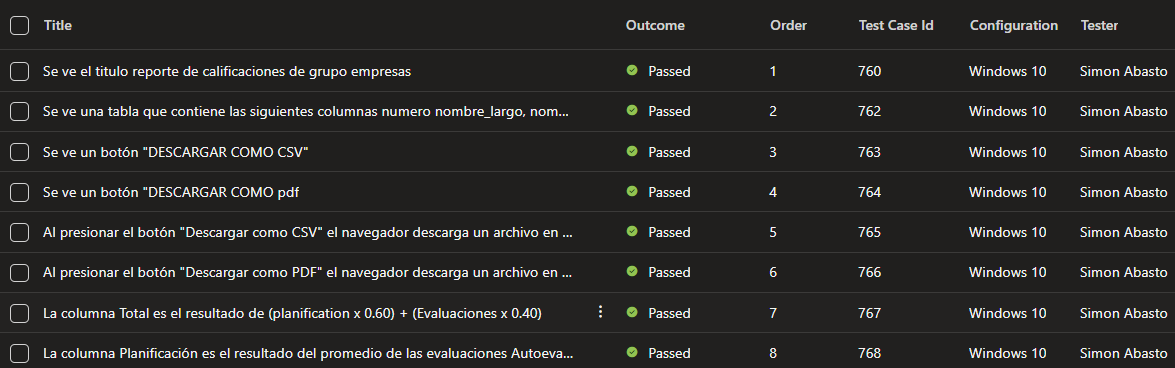
\includegraphics[width=1\linewidth]{Ver reportes de calificaciones de GE.png}
        \caption{Test points Ver reportes de calificaciones de GE}
    \end{figure}

 \begin{table}[h] % Agrega un entorno de tabla
    \centering % Para centrar la tabla en la página
    \caption{Ver reportes de calificaciones de GE} % Agrega la caption aquí
    \begin{tabular}{|c|c|c|c|c|c|}
        \rowcolor{green} % Color de la primera fila
        \hline
        Test plan name & Test points & Run \% & Passed \% & Failed \% & Not run count \\
        \hline
   Ver reportes de calificaciones de GE& 8 & 100 & 100 & 0 & 0 \\
        \hline
    \end{tabular}
\end{table}



%%%%%%%%%%%%%%%%%%%%%%%%%% PRUEBAS
    
    %%%%%%%%%%%%%%%%%%%%%%%%%%%%%%%%%%%%%%%%%%%%%%%%%%%%%%%%%%%%%%%%%%%%%%%%%%%%%%%%%%%%%%%%%%%%%%%%%%%%%%%%%%%%%%%%%%%%%%%%%%%%%%%%%%%%%%%%%%%%%%%%%%%%%%%%%%%%%%%%%%%%%%%%
\section{Resultados de QA}

    \subsection{Métricas de Calidad}
    Todos los 91 Test point fueron ejecutados 
    \\
    el 100\% de pruebas pasadas exitosamente
    
    \subsection{Análisis de los Resultados de Pruebas}
    \begin{figure}[H]
        \centering
        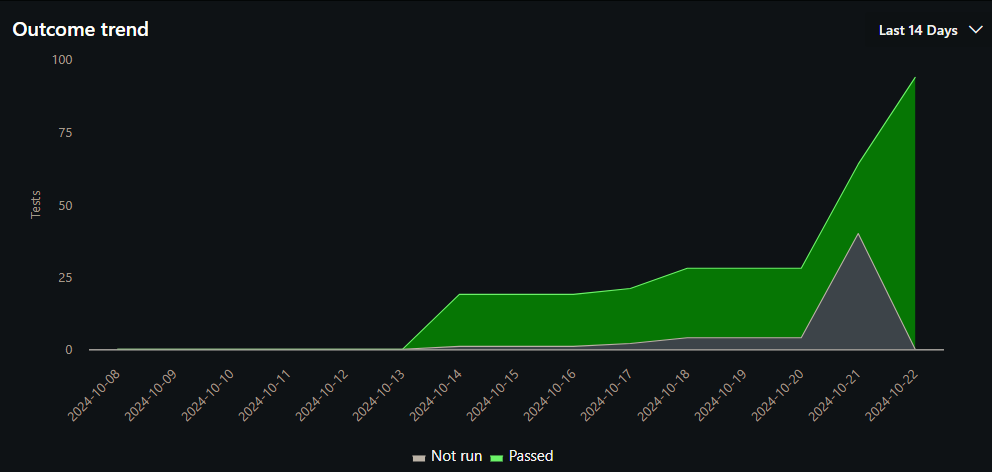
\includegraphics[width=1\linewidth]{grafica.png}
        \caption{Gráfica de pruebas}
    \end{figure}

    \begin{figure}[H]
        \centering
        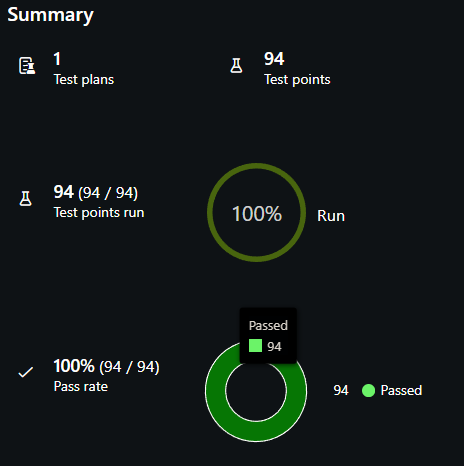
\includegraphics[width=0.5\linewidth]{resumen.png}
        \caption{Resumen de pruebas}
    \end{figure}
    \textbf{Test points totales:} 91\\
    \textbf{Test points Probados:} 91 equivalente a 100\%\\
    \textbf{Test point pasados/aprobados} 91 equivalente a 100\%\\
    \textbf{Test point Fallidos} 0 equivalente a 0\%\\
    \textbf{Test point Bloqueados} 0 equivalente a 0\%\\


    
    Toda la documentación mas detallada esta en DevOps
    
\subsubsection{Resumen total de todos los sprints}
 \begin{figure}[H]
        \centering
        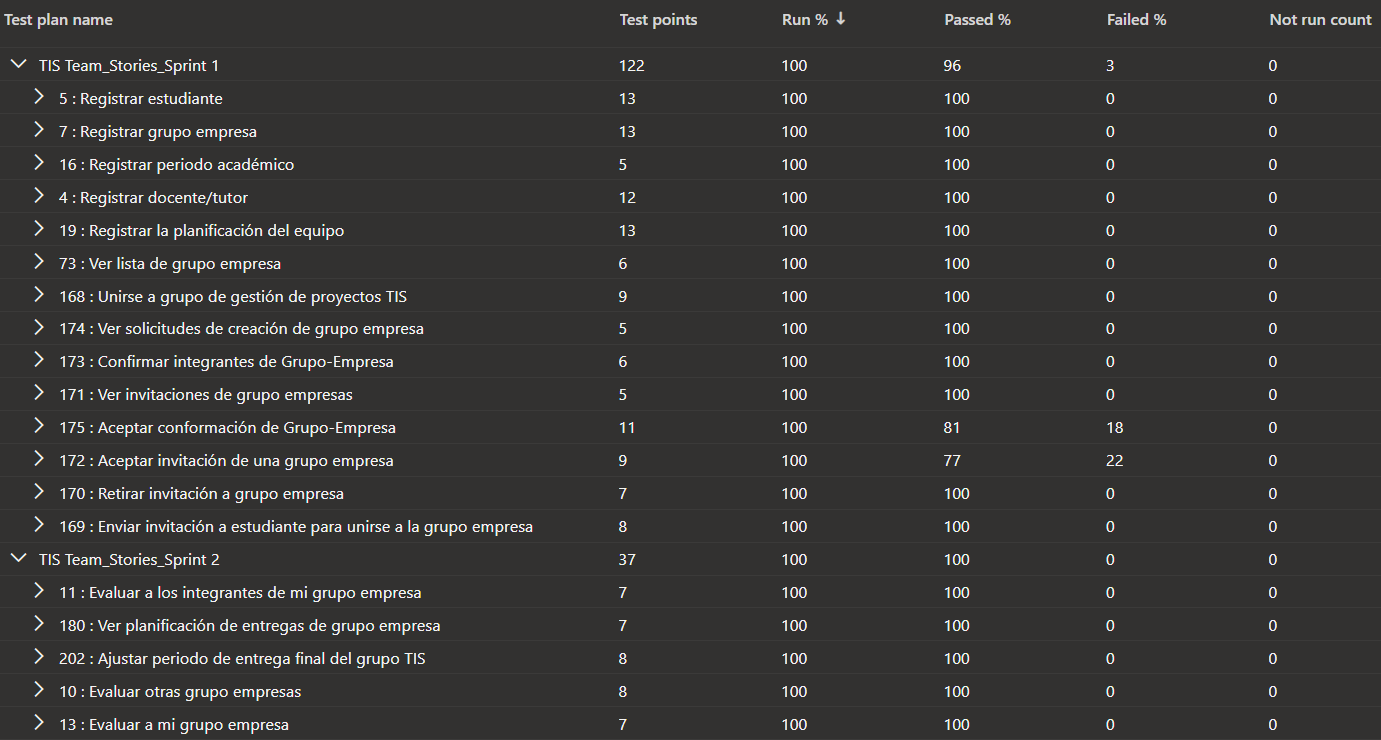
\includegraphics[width=1.13\linewidth]{1.png}
        \caption{Detalles por HU totales}
    \end{figure}

 \begin{figure}[H]
        \centering
        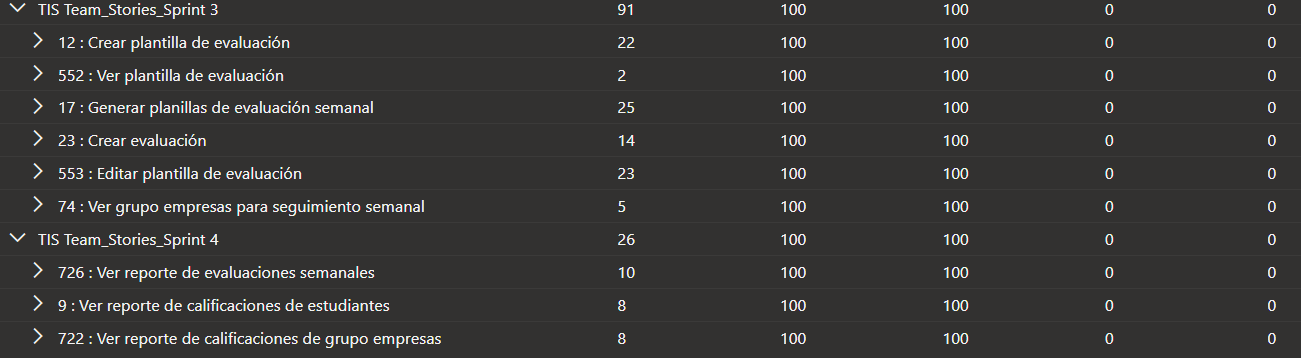
\includegraphics[width=1.13\linewidth]{2.png}
        \caption{Detalles por HU totales}
    \end{figure}






%%%%%%%%%%%%%%%%%%%%%%%%%%%%%%%%%%%%%%%%%%%%%%%%%%%%%%%%%%%%%%%%%%%%%%%%%%%%%%%%%%%%%%%%%%%%
\section{Conclusiones y Recomendaciones}
\begin{itemize}
    \item Cumplimiento de Objetivos: Las pruebas de calidad realizadas han permitido verificar que el software cumple con los objetivos establecidos en el contrato y la adenda correspondiente. Todos los requerimientos funcionales han sido evaluados de manera exhaustiva.
    \item Estabilidad y Confiabilidad: A través de las pruebas ejecutadas, se ha identificado que el sistema presenta un buen nivel de estabilidad y confiabilidad. La mayoría de las funcionalidades han pasado las pruebas con éxito, lo que refleja un software robusto y bien desarrollado.
    \item Rendimiento Aceptable: Las métricas de rendimiento obtenidas durante las pruebas indican que el software opera dentro de los parámetros esperados, con tiempos de respuesta adecuados y un uso eficiente de los recursos del sistema.
    \item Detección de Defectos: Se han documentado y categorizado defectos durante el proceso de QA. Las correcciones de los errores identificados se han priorizado, garantizando que los defectos críticos sean atendidos antes de la entrega final.
    \item Mejoras Recomendadas: Basado en los hallazgos de las pruebas, se sugiere la implementación de mejoras en áreas específicas del software para optimizar aún más su rendimiento y usabilidad. Las recomendaciones se han detallado en el informe de QA.
    \item Importancia de la Documentación: La documentación clara y detallada de los casos de prueba y resultados es crucial para el éxito del proceso de QA. Esta práctica no solo facilita la reproducibilidad de las pruebas, sino que también sirve como referencia para futuras implementaciones y mejoras.
    \item Preparación para Futuras Pruebas: El enfoque adoptado en la planificación y ejecución de pruebas sienta una base sólida para futuras fases de desarrollo. Las lecciones aprendidas durante esta etapa serán valiosas para las próximas iteraciones del proyecto.
    \item Colaboración del Equipo: La participación activa y la colaboración entre los miembros del equipo de QA y desarrollo han sido fundamentales para el éxito de las pruebas. Este enfoque colaborativo debe mantenerse en el futuro para garantizar una comunicación efectiva y resultados de alta calidad.
\end{itemize}

    %\subsection{Conclusiones Generales}
    %\subsection{Recomendaciones para Mejoras Futuras}
    %\subsection{Cambios Propuestos para Futuras Iteraciones}
    %Disminuir la cantidad de HU por sprint para poder tener un control de calidad mas detallado

\section{Referencias}
\begin{enumerate}
    \item  Api Programming Innovators, \emph{Informe de Sprint Backlog del Primer Sprint}.
    \item  Api Programming Innovators, \emph{API Standard for documentation}.
\end{enumerate}



\end{document}

